\documentclass[12pt,a4paper,oneside]{book}
\usepackage{makecell}
\usepackage[left]{lineno}
\usepackage{fancyhdr}%页眉页脚

\headsep 4.3em
\lhead{
\includegraphics[scale=0.08]{polytech.png}}
\chead{}
\rhead{\includegraphics[scale=0.03]{psud.png}}
\lfoot{ZOU Fangzheng}
\cfoot{Polytech Paris-Sud}
\rfoot{\thepage}
%\renewcommand{\headrulewidth}{0.4pt}
%\renewcommand{\footrulewidth}{0.4pt}

\usepackage{xeCJK}  %中文支持
%\usepackage{xunicode,xltxtra}
\usepackage{fontspec}%字体
\usepackage{titlesec}%标题格式
\usepackage[top=2.5cm,bottom=2.5cm,left=2cm,right=2cm]{geometry}%页边距
\usepackage{amsmath}  %数学公式
\usepackage{amssymb}
\usepackage{amscd}
\usepackage{listings}%插入代码
\usepackage{xcolor}  %字体颜色
\usepackage{framed}
\usepackage{lipsum}
\usepackage{color}
\usepackage{graphicx} %插入图片
\usepackage{subfig}  %子图
%\usepackage{subfigure}
\usepackage{tabularx}%插入表格
\usepackage{indentfirst} %首行缩进
\usepackage{array} 
\usepackage{longtable}%长表格
\usepackage{multirow}%使用多栏宏包
%\usepackage{slashbox}
\usepackage{wrapfig}%文字环绕
\usepackage{booktabs} 
\usepackage{extarrows}
\usepackage{ulem}
\usepackage{txfonts}
\usepackage{bm}
\usepackage{cite}%参考文献
\usepackage[super,square,comma,sort&compress]{natbib} 
\usepackage{setspace}%设定行距
\usepackage[colorlinks,linkcolor=black,urlcolor=black,anchorcolor=black,citecolor=black,CJKbookmarks=True]{hyperref}%超链接
%%%listings设置    \begin{lstlisting} !!code!! \end{lstlisting}
\lstset{
        numbers=none, %设置行号位置
       numberstyle=\wuhao, %设置行号大小
        keywordstyle=\color{blue}, %设置关键字颜色
        commentstyle=\color[cmyk]{1,0,1,0}, %设置注释颜色
        %frame=shadowbox, %设置边框格式
        escapeinside=``, %逃逸字符(1左面的键),用于显示中文
        breaklines, %自动折行
        extendedchars=false, %解决代码跨页时,章节标题,页眉等汉字不显示的问题
        xleftmargin=0em,xrightmargin=0em, aboveskip=0.5em,%设置边距
        framextopmargin=0pt,framexbottommargin=2pt,abovecaptionskip=-3pt,
        belowcaptionskip=0pt,  
        %tabsize=1, %设置tab空格数
        showspaces=false %不显示空格
        commentstyle=\color{red!255!green!51!blue!202},%浅灰色的注释  
        keywordstyle=\color{blue!90}\bfseries, %代码关键字的颜色为蓝色,粗体  
        rulesepcolor=\color{red!20!green!20!blue!20},%代码块边框为淡青色  
        stringstyle=\rmfamily\slshape\color[RGB]{128,0,0},
        numberstyle={\color[RGB]{255,1,1}\scriptsize} ,%设置行号的大小,大小有tiny,scriptsize,footnotesize,small,normalsize,large等  
        numbersep=8pt,  %设置行号与代码的距离,默认是5pt  
  basicstyle=\footnotesize, % 这句设置代码的大小  
        frame=shadowbox, %把代码用带有阴影的框圈起来  
        backgroundcolor=\color[RGB]{245,245,244},   %代码背景色         
       }
%表格
\newcommand\mgape[1]{\gape{$\vcenter{\hbox{#1}}$}}  
%中文重定义
\renewcommand{\contentsname}{目录(可以点章节标题,有惊喜)}
\renewcommand{\listfigurename}{插图目录}
\renewcommand{\listtablename}{表格目录}
\renewcommand{\refname}{参考文献}
%\renewcommand{\abstractname}{\sihao\hei 摘\ 要}
\renewcommand{\indexname}{索引}
\renewcommand{\tablename}{表}
\renewcommand{\figurename}{Figure}
\renewcommand{\chaptername}{Chapitre}
\newtheorem{theorem}{定理}
\newtheorem{definition}{\hei 定义}
\newtheorem{property}{问题}
\newtheorem{proposition}{猜测}
\newtheorem{lemma}{引理}
\newtheorem{corollary}{推论}
%设置主字体
\setCJKmainfont{Microsoft YaHei}
\setmainfont{Segoe UI Semilight}
%\setmainfont{Courier New}
%\setmainfont{DejaVu Serif} 
%\setmainfont{Palatino Linotype} 
%字号
\newcommand{\ziding}{\fontsize{50pt}{\baselineskip}\selectfont}%自定义大号
\newcommand{\yihao}{\fontsize{26pt}{\baselineskip}\selectfont}%二号
\newcommand{\erhao}{\fontsize{22pt}{\baselineskip}\selectfont}%二号
\newcommand{\xiaoer}{\fontsize{18pt}{\baselineskip}\selectfont}%小二
\newcommand{\sanhao}{\fontsize{16pt}{\baselineskip}\selectfont}%三号
\newcommand{\xiaosan}{\fontsize{15pt}{\baselineskip}\selectfont}%小三
\newcommand{\sihao}{\fontsize{14pt}{\baselineskip}\selectfont}%四号
\newcommand{\xiaosi}{\fontsize{12pt}{\baselineskip}\selectfont}%小四
\newcommand{\wuhao}{\fontsize{10.5pt}{\baselineskip}\selectfont}%五号
\newcommand{\xiaowu}{\fontsize{9pt}{\baselineskip}\selectfont}%小五
\titleformat{\section}{\bfseries\centering\sihao\yhei}{\thesection}{1em}{}
\titleformat{\subsection}{\sihao\yhei}{\thesubsection}{1em}{}
\titleformat{\subsubsection}{\xiaosi\yhei}{\thesubsubsection}{1em}{}
\titleformat{\chapter}{\bfseries\centering\sanhao\arbd}{\thechapter}{1em}{}
%\titleformat{\part}{\centering\sanhao\hei}{第\,\thepart\,章}{1em}{}
%中文断行
\XeTeXlinebreaklocale "zh"
\XeTeXlinebreakskip = 0pt plus 1pt minus 0.1pt
%设置字体
%\newfontfamily\song{SimSun}
%\newfontfamily\hei{SimHei}
%\newfontfamily\fangsong{FangSong}
%\newfontfamily\kai{KaiTi}
\newfontfamily\timesnew{Times New Roman}
\newfontfamily\cons{Consolas}
\newfontfamily\deja{DejaVu Serif}
\newfontfamily\segoe{Segoe UI Semilight}
\newfontfamily\arbd{Arial Bold}
\newfontfamily\bkmo{Bookman Old Style}
\newfontfamily\yhei{Microsoft YaHei}
\newfontfamily\yhui{Microsoft YaHei Light}
\newfontfamily\ftin {Fontin SmallCaps}
\newfontfamily\pala {Palatino Linotype} 
%我自己设置的字体
\setCJKfamilyfont{zhsong}{SimSun}
\setCJKfamilyfont{zhhei}{SimHei}
\setCJKfamilyfont{zhfs}{FangSong}
\setCJKfamilyfont{zhkai}{KaiTi}
\newcommand*{\song}{\CJKfamily{zhsong}} % 宋体
\newcommand*{\hei}{\CJKfamily{zhhei}}   % 黑体
\newcommand*{\kai}{\CJKfamily{zhkai}}  % 楷书
\newcommand*{\fangsong}{\CJKfamily{zhfs}}  % 仿宋

%行段间距
\linespread{1.2} %行间距
\setlength{\parskip}{2.3\baselineskip}%段间距
%重定义
\newcommand{\enmainfont}{\timesnew}
\newcommand{\zhmainfont}{\song}
\newcommand{\ud}{\mathrm{d}}          %用\ud 作为微分算子“d”
\newcommand{\inti}{\int_{-\infty}^{+\infty}}%无穷积分

\newcommand{\en}[1]{\enmainfont{#1}\zhmainfont}
\newcommand{\zh}[1]{\zhmainfont{#1}\enmainfont}
\newcommand{\drop}{ 0.08\textheight}
%%数学公式设置
\setlength{\abovedisplayskip}{50pt}    
\setlength{\belowdisplayskip}{60pt}
%\renewcommand{\arraystretch}{1.3}   %將表格行間距加大為原來的  倍
%\setlength{\abovecaptionskip}{10pt}%对图片是标题上方的间距,对表格是标题下方的间距
%\setlength{\belowcaptionskip}{0pt}%对图片是下方,对表格是上方
%\setlength{\parindent}{2.45em}  %首行缩进
\definecolor{shadecolor}{rgb}{0.92,0.92,0.92}
%%%%%%%%%%%%%%%%%%%%%%%%%%%%%%%%%%%%%%%%%%%%%%%%%%%%%%%%%%%%%%%%%%%%%%%%%%%%
\setlength\parindent{0pt}
\begin{document} \sihao
\begin{minipage}{0.2\textwidth}
%
\hspace*{0.2\textwidth}\textcolor[RGB]{16,136,136}{\rule{6pt}{\textheight}}
\end{minipage}
\hfill
\begin{minipage}{0.8\textwidth}

\thispagestyle{empty}
\par
\par

\vspace*{0.2\textwidth}
\hspace*{0.3\textwidth}
{\bfseries \yihao \bkmo\textcolor[RGB]{181,72,61}{\LaTeX 新手攻略}}\\[\drop]
\vspace*{0.02\textwidth}
\hspace*{0.6\textwidth}
BY {\sihao\bkmo 邹方正}\\
\vspace*{0.02\textwidth}
\hspace*{0.3\textwidth}
{\small \deja \textcolor[RGB]{20,144,188}{FANGZHENG.ZOU@GMAIL.COM}}\\
\vfill
\begin{center}

\includegraphics[scale=0.15]{latex.png}
\end{center}
\vspace*{0.1\textwidth}
\begin{center}
A Massy, mercredi le 4 novembre.
\end{center}
\end{minipage}
\restoregeometry
\setcounter{page}{1}
\tableofcontents

\newpage
\setcounter{page}{1}
\chapter{下载安装}



\section{语言引擎安装}
一定要 \textcolor[RGB]{255,0,51} {先下载}这个语言引擎!
\par
一定要 \textcolor[RGB]{255,0,51} {先下载}这个语言引擎!
\par
一定要 \textcolor[RGB]{255,0,51} {先下载}这个语言引擎!
\par

win版地址:\href{http://pan.baidu.com/share/link?uk=705221041&shareid=72337831&third=0&adapt=pc&from=wapforcetoweb}{点我打开}

mac版地址:\href{http://pan.baidu.com/share/link?uk=2064390295&shareid=584901926&third=0&adapt=pc&fr=ftw}{点我打开}


\par

然后用虚拟光驱加载安装,安装文件是这个:
\par

\begin{figure}[htp] 
\centering 
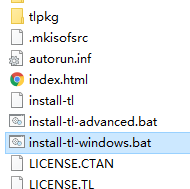
\includegraphics[scale=0.75]{tl.png}
\caption{安装文件}%`图片的标题`
\label{pic:tl}
\end{figure}
\vspace{2em}

\section{编译器安装}
\par
然后再安装这编译器:地址:\href{http://www.xm1math.net/texmaker/download.html}{点我打开}

\par
我使用TexMaker,因为可以很好的支持XeLaTex。不推荐其他引擎+编译器组合,因为XeLaTex已经十分优秀(还直接支持中文),使用又简单。
\par
然后我们就可以开始写 报 告 了OwO !!
\chapter{总览介绍}
\begin{center}
\LaTeX {\bfseries {很简单!}}
\end{center}
\vspace{2em}
\section{LaTeX语言}
\LaTeX 是一种{\color{cyan}标签语言},类似html,就是简单地在需要处理的文字前面加上指令就可以了。并且,有相当多的排版系统已经预先设定好了,我们做的大多数工作就是往里面填写报告内容。
\par
Q:那需要背很多指令吗? A:{\color{cyan}不用}!在后面会讲到。
\par
但是,刚上手的小伙伴可能会被虐到,因为习惯了Office系列的鼠标操作。你会发现在\LaTeX 的世界不管要做什么都得靠{\color{cyan}代码}。就算另起自然段这种操作,都要通过输入 $\backslash$par 来实现……
\par
但是不要担心,因为有了秘笈……
\section{TexMaker介绍}
这是一款不错的编译器,但是我还没研究怎么让它对除了英语的其它语言进行查错。(不要紧)
\par
有一个很重要的设置,就是选择编译环境。依次点击【选项】-【配置TexMaker】-左边【快速构建】
\par
\begin{figure}[htp] 
\centering 
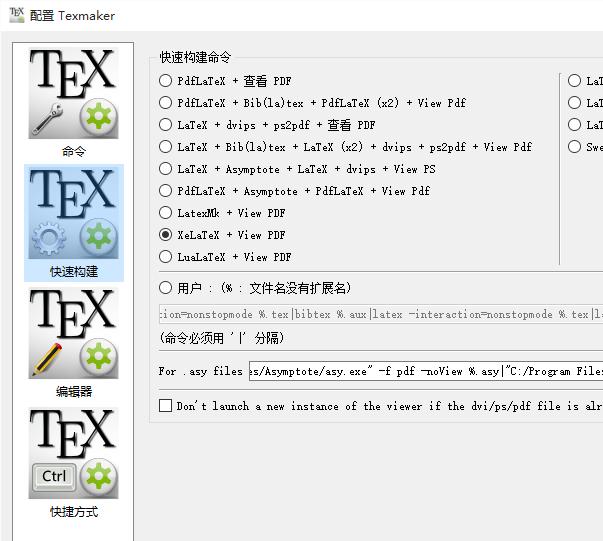
\includegraphics[scale=0.45]{tm.png}
\caption{选择组合}%`图片的标题`
\label{pic:tm}
\end{figure}

\par
如刚才所说,{\color{cyan} 一定要选择}XeLaTex+View PDF这个组合。
\par
这款编辑器有一个优点,就是你自己电脑上已经安装的字体,可以直接使用。在头文件区域里面添加指令
\par
\begin{lstlisting}[language={[ANSI]C}, numbers=left, numberstyle=\tiny, keywordstyle=\color{blue!70},  frame=shadowbox, rulesepcolor=\color{red!20!green!20!blue!20}]
\newfontfamily\cons{Consolas} // \cons是你任意取的名字,正文区域可以当作指令使用
\end{lstlisting}
\par

\chapter{功能介绍}
\section{基本情况}
每篇文章的结构都是{\color{magenta}头文件区域}+\textcolor[RGB]{90,90,90}{正文区域}。
\par
在头文件区域里面要给出缺省设置和加载库。(不必纠结于此)正文区域以$\backslash$begin \{document\} 和 $\backslash$end\{document\}为起止点。
\par
这篇小教程的Tex头文件区域是我每次写报告都会使用的,已经被我增加到160行左右,含有平时写报告必备的库和设置。(复制走吧!)
\par
\LaTeX 的指令都是以$\backslash$开头,注释以 \% 开头
\par

{\bfseries {下面来举一个实际例子。}}
\par
就拿上面这句话来说,它加粗了,是这样实现的。
\par
{\cons 
\begin{lstlisting}[numbers=left, numberstyle=\tiny, keywordstyle=\color{blue!70},  frame=shadowbox, rulesepcolor=\color{red!20!green!20!blue!20}]
{\bfseries {下面来举一个实际例子。}}
\end{lstlisting}
\par
$\backslash$bfseries 的意思是加粗。所以你明白了嘛?
\par
又一个栗子:
\par
{\textit {\textcolor[RGB]{20,200,145} {Polytech Paris-Sud}}}
\par
这句话字体倾斜,颜色变了,是这样实现的。
\par

\begin{lstlisting}[language={[ANSI]C}, numbers=left, numberstyle=\tiny, keywordstyle=\color{blue!70},  frame=shadowbox, rulesepcolor=\color{red!20!green!20!blue!20}]
{\textit {\textcolor[RGB]{20,200,145} {Polytech Paris-Sud}}}
\end{lstlisting}
\par
$\backslash$textit 表示斜体, $\backslash$textcolor[RGB]$\{$20,200,145$\}$ 表示XXX颜色。

\par
\LaTeX 的处理文字方式跟上面的例子大同小异,注意好大括号的层次,别对不上就可以了。
\vspace{2em}
\section{图片摆放}
\LaTeX 里图片的设置稍微复杂,但是功能也更强大。
\par
本文上之前的图片都是用这一段代码插入的。例如\ref{pic:tm}(点击标号可以跳转)
\par
\begin{lstlisting}[language={[ANSI]C}, numbers=left, numberstyle=\tiny, keywordstyle=\color{blue!70},  frame=shadowbox, rulesepcolor=\color{red!20!green!20!blue!20}]
\begin{figure}[htp] //h=here,t=top,p=page 这些是让系统自动选择图片最合适的位置
\centering //居中
\includegraphics[scale=0.45]{文件名.png} //这里表示设置为原图尺寸的45%
\caption{图片说明}% 
\label{pic:图片标签} //超链接用
\end{figure}
\end{lstlisting}
\par
可以把需要插入的图片就放在跟Tex文件相同的目录下,图片文件名改得简单一点。
\par
还有一种常用的,并排放两张图的方式,给出代码~
\par
\begin{lstlisting}[language={[ANSI]C}, numbers=left, numberstyle=\tiny, keywordstyle=\color{blue!70},  frame=shadowbox, rulesepcolor=\color{red!20!green!20!blue!20}]
\begin{figure}[h]
\centering
\includegraphics[scale=0.66]{图片一.png}
\includegraphics[scale=0.66]{图片二.png}
\caption{嘻嘻嘻}
\label{pic:哈哈哈}
\end{figure}
\end{lstlisting}
\par
效果就是这样:
\par
\begin{figure}[h]
\centering

\includegraphics[scale=0.21]{tr.png}

\includegraphics[scale=0.21]{xf.png}
\caption{两张图水平并排共享标题}
\label{pic:dora}
\end{figure}
\par
至于想像Word一样,采取文字环绕图片等等版式,我只想说,这就是Word生成的PDF杂乱无章的罪魁祸首,还是不要用了,并不会漂亮多少的。
\vspace{2em}
\section{绘制表格}
我的建议是,如果表格比较复杂,不要用\LaTeX 绘制,用Word画好截图放进来。
\par
简单的表格画法:
\par
\begin{center}
\begin{tabular}{r|cl|}
\hline
1111&dff&fzg8\\
\hline
222&fez&fgegz\\
333333&&ggg\\
\end{tabular}
\end{center}

\par
这是一个例子,代码如下:

\par

\begin{lstlisting}[language={[ANSI]C}, numbers=left, numberstyle=\tiny, keywordstyle=\color{blue!70},  frame=shadowbox, rulesepcolor=\color{red!20!green!20!blue!20}]
\begin{tabular}{r|cl|} /*设置列数,并同时指定对齐方式和确定列框线,这里为
三列,第一列右对齐,第二列居中,第三列左对齐,同时第一列右侧有列框线
第三列右侧有列框线。(r=right,c=center,l=left)*/
\hline //画一条横框线
1111&dff&fzg\\ /*每一行从左至右填写表格内容,单元格之间用&隔开
每行结束用 \\表示*/
\hline //画一条横框线
222&fez&fgegz\\ //没有画横框线 所以结果里也没有
333333&&ggg //单元格可以没有内容,但是&不能少
\end{tabular}
\end{lstlisting}
\par
至于像下面这种含有合并单元格,精确画格线的表格,请结合代码并谷歌 “makecell latex”。

\par
\begin{center}
\begin{tabular}{rrrr}
\Xhline {1.0pt}
\multicolumn{1}{!{\vrule width1.2pt}c!{\vrule width0.7pt}}{\multirow {3}{*}{\mgape{
\includegraphics[scale=0.3]{polytech.png}}}}&\multicolumn{2}{c}
{ \erhao \song Rapport du TP3}&\multicolumn{1}{!{\vrule width0.7pt}c!{\vrule width1.2pt}}{\deja Et3 - EES}
\\
\Xcline{4-4}{0.5pt}
\multicolumn{1}{!{\vrule width1.2pt}c!{\vrule width0.7pt}}{} &\multicolumn{2}{c}
{\slshape \sffamily \sihao Matière: Réseaux}& \multicolumn{1}{!{\vrule width0.7pt}c!{\vrule width1.2pt}}{ \deja jeudi le}
\\ 
\multicolumn{1}{!{\vrule width1.2pt}c!{\vrule width0.7pt}}{} &\multicolumn{2}{c}
{\deja \bfseries \small ZOU Fangzheng / YANG Pantao} &
\multicolumn{1}{!{\vrule width0.7pt}c!{\vrule width1.2pt}}{\deja 18/06/2015}
\\
\Xhline {1.2pt}
\end{tabular}
\end{center}

\par
代码如下:
\par

\begin{lstlisting}[language={[ANSI]C}, numbers=left, numberstyle=\tiny, keywordstyle=\color{blue!70},  frame=shadowbox, rulesepcolor=\color{red!20!green!20!blue!20}]
\begin{tabular}{rrrr}
\Xhline {1.0pt}
\multicolumn{1}{!{\vrule width1.2pt}c!{\vrule width0.7pt}}{\multirow {3}{*}{\mgape{
\includegraphics[scale=0.3]{polytech.png}}}}&\multicolumn{2}{c}
{ \erhao \song Rapport du TP3}&\multicolumn{1}{!{\vrule width0.7pt}c!{\vrule width1.2pt}}{\deja Et3 - EES}
\\
\Xcline{4-4}{0.5pt}
\multicolumn{1}{!{\vrule width1.2pt}c!{\vrule width0.7pt}}{} &\multicolumn{2}{c}
{\slshape \sffamily \sihao Matière: Réseaux}& \multicolumn{1}{!{\vrule width0.7pt}c!{\vrule width1.2pt}}{ \deja jeudi le}
\\ 
\multicolumn{1}{!{\vrule width1.2pt}c!{\vrule width0.7pt}}{} &\multicolumn{2}{c}
{\deja \bfseries \small ZOU Fangzheng / YANG Pantao} &
\multicolumn{1}{!{\vrule width0.7pt}c!{\vrule width1.2pt}}{\deja 18/06/2015}
\\
\Xhline {1.2pt}
\end{tabular}
\end{lstlisting}
\par

挺麻烦的,不如画好了截图放进来(真心话).
\vspace{2em}
\section{插入代码}
你可能已经发现了,这代码贴得挺别致的:
\par
\begin{lstlisting}[language={[ANSI]C}, numbers=left, numberstyle=\tiny, keywordstyle=\color{blue!70},  frame=shadowbox, rulesepcolor=\color{red!20!green!20!blue!20}]
#include <stdio.h>
#define V_MAX 3.0f
#include <string.h>
int main()
{
    char a[33];
    scanf("%s",&a); //input a string
    printf("len=%dn",strlen(a));
}
\end{lstlisting}
\par
所用的\LaTeX 代码如下:
\par
\begin{lstlisting}[language={[ANSI]C}, numbers=left, numberstyle=\tiny, keywordstyle=\color{blue!70},  frame=shadowbox, rulesepcolor=\color{red!20!green!20!blue!20}]
`$\backslash$`begin{lstlisting}[language={[ANSI]C}, numbers=left, numberstyle=\tiny, keywordstyle=\color{blue!70},  frame=shadowbox, rulesepcolor=\color{red!20!green!20!blue!20}]
【代码段】
`$\backslash$`end{lstlisting}


\end{lstlisting}
\par
所以需要贴代码的时候,把代码换到【代码段】位置就可以了。

\chapter{进阶技能}
\section{插入公式}
推荐一个网站,无需手动输入,只要鼠标啪啪啪点就可以了。
\par
地址:\href{http://www.codecogs.com/latex/eqneditor.php}{点我打开}
\par

跟数学有关的东西,都需要用两个美元符号括起来。在编辑器中会自动变成绿色。\$ 数学语句 \$
\par
例如这样的一组公式在刚才的网页上可以轻松完成。
$
\left\{\begin{matrix}\begin{array}{rcl}

\dot{u}&=&vr+\tau _{u}\\
&\\
\dot{v}&=&-ur\\
&\\
\dot{r}&=&\tau _{r}\\

\end{array}\end{matrix}\right.
$

\chapter{重要秘籍}
说一个很重要,很有用,很高效,很酸爽的秘籍。

\par
之前说,不需要记忆很多指令,是因为我们可以自定义快捷指令,在这里:
\par
\begin{figure}[htp] 
\centering 
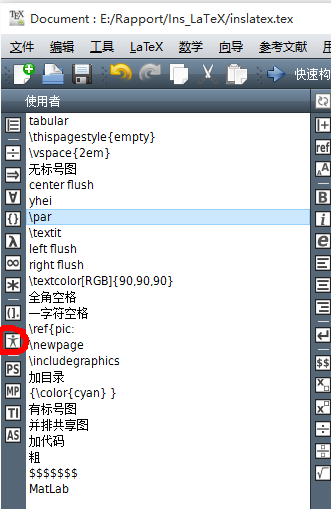
\includegraphics[scale=0.85]{is.png}
\caption{TexMaker的这里}%`图片的标题`
\label{pic:is}
\end{figure}
\par
你可以添加许多常用的指令,比如换行,加粗,居中,画表格,贴代码……到那时候,你的LaTeX速度就起飞了。
\par
这里给出我常用的一些指令:(只能手动一个一个添加)
\par
\begin{lstlisting}[language={[ANSI]C}, numbers=left, numberstyle=\tiny, keywordstyle=\color{blue!70},  frame=shadowbox, rulesepcolor=\color{red!20!green!20!blue!20}]
画表格:
\begin{tabular}{rl}

\end{tabular}

添加目录:
\tableofcontents

清除本页格式:
\thispagestyle{empty}

回车两行:
\vspace{2em}

简单插图:
\includegraphics[scale=0.3]{111.png}

无标号图:
\begin{figure}[htp] 
\centering 
\includegraphics[scale=0.45]{.png}
\caption*{}%
\label{pic:pol}
\end{figure}

有标号图:
\begin{figure}[htp] 
\centering 
\includegraphics[scale=0.45]{.png}
\caption{}%
\label{pic:}
\end{figure}

并排共享标题图:
\begin{figure}[h]
\centering
\includegraphics[scale=0.66]{etop.png}
\includegraphics[scale=0.66]{ebot.png}
\caption{  }
\label{pic:fig1}
\end{figure}


居中:
\begin{center}

\end{center}

居左:
\begin{flushleft}

\end{flushleft}

居右:
\begin{flushright}

\end{flushright}

修改颜色(RGB)
\textcolor[RGB]{90,90,90}{ }

斜体:
\textit { }

全角空格:
\quad 

半角空格:
\  //斜杠和一个空格


另起一页:
\newpage

另起一段:
\par


\end{lstlisting}
\par
\chapter{推荐网站}
直接点击:
\par
\href{https://github.com/ayucapal/ins_LaTeX.git}{本教程GitHub}
\par

\LaTeX \href{http://www.codecogs.com/latex/eqneditor.php}{官方Guide}
\par
\href{https://openclassrooms.com/forum/sujet/formulaire-de-formules-latex-84687}{数学符号查询输入表}
\par
\href{http://home.deib.polimi.it/mredaelli/circuitikz/index.html}{TikZ画电路图}
\par
\href{http://www.ctex.org/documents/latex/graphics/node20.html}{插图指令集}
\par

\href{http://www.cs.pu.edu.tw/~wckuo/doc/latex123/node9.html}{表格处理教程}
\par

\href{https://bitbucket.org/rivanvx/beamer/wiki/Home}{Beamer:用\LaTeX 制作PPT}
\chapter{更新日志}
11/11/2015 更新:
\par
特别感谢张子谋同志,是他的\LaTeX 贴心教程 给我启蒙。我的绝大部分技能都是从这份教程里面获得的。
\par
如果你发现使用加粗、倾斜等命令后没有效果,很有可能是你选择的这句话字体本身不带加粗、倾斜效果。
\par
在GIT同目录下,有一些说明文档(PDF格式),详情请参见Git下README文件。
\par

04/11/2015 更新:
\par

如果你发现copy了我的头文件区域之后不能compiler,十有八九是因为我用过的字体在你的电脑里没有安装。
\par
初使用\LaTeX 的一段时间必然是挺痛苦的 但是越写越带劲~加油小伙伴们!
\par
\begin{flushright}
邹方正
\end{flushright}
\end{document}